\chapter{Orchestration}

\section{General Context}
IoT initially had two visions, one is \textit{Internet oriented} vision and another one is \textit{Things oriented} vision. Later when new challenges introduced such as unique addressing and storing information, \emph{Semantic oriented} vision had arisen \cite{IoT:Survey}. According to the orientation, the participating devices are categorised and the orchestration is configured. In smart-phones, all the visions are exists. 
\subsection{IoT elements of smartphones}
In \cite{IoT:Arch}, the general architecture of IoT is well explained as four layers. \emph{Perception Layer} is where all the information collected, say, from the environment using specialised equipments such as sensors and GPS. Thus this layer provides the digital representation of physical world. \emph{Network Layer} is for communication and transmission of information. \emph{Middle-ware Layer} by its various intelligent cloud computing supports the application layer and act as a intermediate between network layer and application layer. \emph{Application Layer} is fully customized with respect to the users and the purpose of the application. In some scenarios, both the perception layer and application layer reside in the same smart-phone system.
\subsection{Need for orchestration}
The main goal is to provide energy efficient decision(s) back to the service enabled smart-phones which are participating in the Orchestration. Orchestration, the concept existing in the music world was adopted in the process automation of business world by automating, coordinating and managing complex systems, middle-wares and services. In the context of vulnerability to energy efficiency, even a single piece of code  ( {\tt while(battery.percentage) println(battery.percentage)}) could be potentially dangerous, leading any effort made to find suboptimal solutions into vain. Hence, there is a need for the great intelligent system, which is capable of finding and categorizing the energy errors. The system should have access to powerful \textit{dynamic control system engine} for fixing such errors. To assist bug fixing we may need a strong insights from the big data of crowd sourced logs/operations  over the time. The big data may lead to \emph{side-effect services} (new enabling services other than energy-efficiency). Hence the energy and effort of making this grant system has huge benefits in return. Thus the \emph{Orchestration}  with the capabilities of integrating different types of clouds, processes and services is an suitable choice. 

\subsection{Composition of systems and models and services}
\begin{figure}[h]
 \begin{center}
 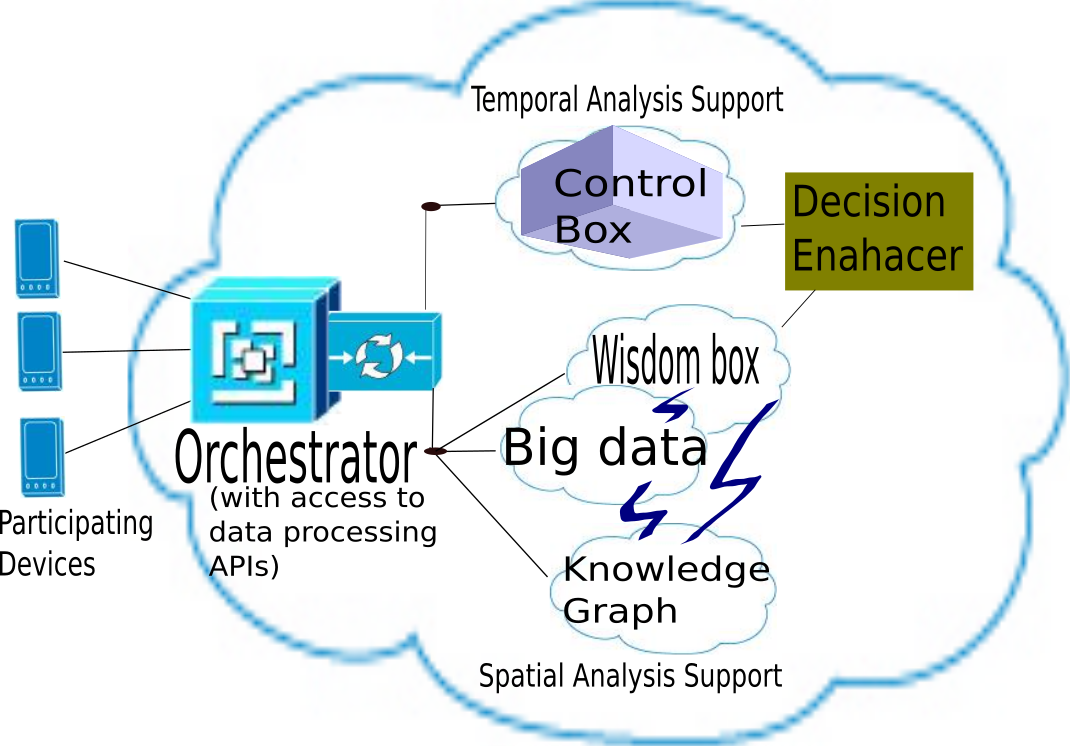
\includegraphics[scale=0.30]{Figures/EEaaOSArchEnhanced.png}
 \end{center}
 \caption{EEaaS Orchestration}
 \label{fig:Orch}
\end{figure}

We propose an architecture design of orchestrator as depicted in Figure \ref{fig:Orch}, with the primary understanding of the participating systems. Then to evaluate and enhance, any existing reference models or relevant solutions in the other related domains may be adopted in the future. The design is open and flexible which make it possible to add,remove and merge number of \textit{systems, models and services} at any granular level in the orchestrator. The orchestrator organizes the following components, \emph{Participating Devices}, \emph{Data Processor}, \emph{Big data storage}, \emph{Knowledge graph}, \emph{Wisdom box}, \emph{Control box} and  \emph{Decision Enhancer} % and \emph{Error Sack}.
\subsubsection{Participating devices}
\label{subsection:partdevice}
These are the devices interested in optimized energy usage. Upon registration with orchestrator, a dark skinned, fully customizable, lower energy consuming background \textit{service application} is enabled in the devices. This application sends low level system-call logs periodically and reports strange system behaviours spontaneously. To avoid security and privacy issues, logs are collected anonymously with unique device profile. This application not only a logs collector, it will also act as local \textit{self-controller}, try to catch energy errors in-time and its functionalities are regularly updated by orchestrator. This is to avoid the need of continuous data communication. 
\subsubsection{Data processor}
Data processor is a collection of APIs for various data processing methods accessible to orchestrator. According to the context, methods will be chosen by the orchestrator. Here the data is processed for both big data analysis and temporal analysis.
\subsubsection{Big data storage and modern tools}
The data produced by smart-phones would be in massive scale over the time. Thus to handle this data-intensiveness we require big data storage and modern cloud programming paradigms such as \emph{Hadoop} and \emph{Apache flink}. For deep analysis of sample data, powerful  computing languages such as \emph{Python} and \emph{R} are required.
\subsubsection{Knowledge graph}
By referring the big data of logs, dynamic knowledge graph is built and then keep on updated. Nodes are qualified classes and subclasses with attribute-value pairs. So it provides a clear and structured view of data. Using this graph, it is then easy to get specific data for analysis with respect to location, device model, internet service provider and for various specification.
% reference is better than saving a copy of graph data 
\subsubsection{Wisdom box}
Wisdom box contains set of learners whose primary focus is building location specific insights (spatial domain). The box act as a predictor of trends in data, usage patterns, system behaviour anomalies. It uses combination of statistical algorithms and machine learning algorithms to find energy efficient decisions. The decisions that are independent of device, platform and applications is stored in \emph{Decision Enhancer} in the orchestration. Device, platform and applications specific decisions fused in the knowledge graph and the reference graph stored in the decision enhancer. 
\subsubsection{Control box}
Control box is a builder of real-time self-controllers for the participating \textit{dynamic systems} with the help of time-sensitive feedbacks (temporal domain). These self-controllers embedded as a service as explained before in \ref{subsection:partdevice}. To make these self-controllers even better, context related decisions in spatial domain are used. Feedbacks are received from the participating devices to evaluate the performance along with log collection.

%% --------Excess -----%
%In this section we would like to highlight some key concepts which is really important to understand our navally proposed cloud orchestration for energy efficiency. First we explain the system architecture of IoT in general and specify that of smartphone . Then the suitable mathematical models from the field of control system theory which deals with dynamic systems.

%fog computing\\
%cloud os\\
%integration of types of clouds\\
%automation\\
%distributed computing

%Internet is constantly evolving phenomenon so is IoT. Hence the problem solver must 
%have best capabilities with respect to the system of devices it deals with including 
%\begin{itemize}
%\item quickly identifies the system
%\item 
%\end{itemize}
%ready to embrace  future changes and flexible. To simply put it , it should have best learning capacity of the system it deals with and  


%Green networking is the practice of selecting energy-efficient networking technologies and products, and minimizing resource use whenever possible.

%https://sites.google.com/site/simulationarchitecture/jeqn
%https://en.wikipedia.org/wiki/Simulink\\

%\subsubsection{Error sack}
%It is in essence reference dictionary of error values for {\tt (input, output)} pairs. For efficiency,the values are received along with next patch of logs. Hence except for the fist time, the participating devices periodically send the logs along with the error values for the previous output signals.
%
%To make the orchestration more efficient, except the participating devices, all other components completely connected thus by improving smartness of the orchestrator to react quickly in case of invalid data inputs and redundancy  and to  achieve some special tasks.